\chapter{Physics of Z Transverse Momentum}
\label{chapter:theory}

\section{The Standard Model}
\label{section:standard_model}

Our current understanding of how matter interacts at high energies is entirely
described by the standard model as constructed by Weinberg, Glashow, and
Salam \cite{glashow1961}\cite{weinberg1967}\cite{salam1968}. The model combines
three of the four fundamental forces (leaving out only gravity, which is so
weak as to be negligible) and is the most accurate and best tested scientific
theory ever formulated.

\subsection{The Electromagnetic Force}
\label{subsection:electronmagnetic_force}

The modern theory of electromagnetism began with Maxwell's theory developed in
the middle of the 19th century \cite{maxwell1873}. Maxwell was the first to
conclude that light was an electromagnetic wave, the full importance of which
was only later understood when it was discovered that the photon was the force
carrier of the electromagnetic force \cite{maxwell1865}.

In the early 20th century, Lorentz and Einstein developed relativistic
mechanics and showed that Maxwell's theory was Lorentz invariant
\cite{lorentz1899}\cite{einstein1904}. Dirac updated the theory in 1920 when he
was able to quantize the electromagnetic field as an ensemble of harmonic
oscillators \cite{dirac1927}. Dirac would go on to discover that anti-particles
were a natural consequences of his equations \cite{dirac1928}\cite{dirac1930}.
These anti-particles were found by Anderson in 1932 as he observed cosmic rays
in a cloud chamber \cite{anderson1933}.

As microwave technology improved in the 1940s, more accurate measurements of
the energy level shifts in hydrogen were made, resulting in the discovery of
the Lamb shift by Lamb and Rutherford \cite{lamb1947}. This discovery pointed
to discrepancies in the theory. Bethe would resolve these discrepancies by
showing that the theory could account for the Lamb shift using non-relativistic
calculations \cite{bethe1947}. Bethe's work inspired multiple other physicist
including Dyson, Feynman, Schwinger, and Tomonaga to work along similar lines.
They created quantum electrodynamics (QED), a fully relativistic and
self-consistent theory of electromagnetic interactions
\cite{tomonaga1946}\cite{schwinger1948}\cite{feynman1949}\cite{dyson1949}.

QED is a perturbation theory with expansions performed in terms of the fine
structure constant, \fsc. As $\fsc \approx 7.297 \cdot 10^{-3}$, the higher
order terms contribute smaller and smaller corrections and so only a few orders
need to be computed to make very accurate predictions. For example, the
anomalous magnetic moment of the electron is calculated to $\fsc^{4}$, and
agrees with experiment to more than 10 significant figures.

\subsection{The Weak Force}
\label{subsection:weak_force}

The need for a weak force, and hence a theory describing it, was first hinted
at by beta decay experiments in the early 1900s. These experiments culminated,
in 1914, in Chadwick's discovery that the energy spectrum of electrons ejected
in beta decay was continuous instead of a delta function as would be expected
for a two-body decay \cite{chadwick1914}. While some proposed that this
discovery indicated that momentum and energy were not conserved, Pauli proposed
an alternative: there was a neutral and invisible particle that carried away
some of the energy---the neutrino \cite{pauli1930}. Fermi began working on this
idea and invented a four fermion contact interaction in which a neutron decayed
into a proton, an electron, and a neutrino \cite{fermi1934}.

In 1947, Rochester and Butler discovered a particle that decayed to two pions
which they called the $\theta$; in 1949, Brown and Powell discovered a particle
that decayed to three pions which they called the $\tau$
\cite{Rochester1947}\cite{brown1949}. It was soon discovered that these
particles had the same mass and lifetime---indicating that they were the same
particle---but, based on their decay products, they must have different parity.
Lee and Yang proposed that the $\theta$ and the $\tau$ were in fact the same
particle, but that it was undergoing a parity violating decay \cite{lee1956}.
Their idea was confirmed by Wu in 1956, who showed that electrons were
preferential emitted from \cobaltsixty in one direction, and by Garwin,
Lederman, and Weinrich in 1957, who studied \pitomunu decays in a storage ring
\cite{wu1956}\cite{garwin1957}.

In 1954, Yang and Mills replaced Fermi's contact interaction with a non-Abelian
gauge theory that contained a spin-1 boson to mediate the force
\cite{yang1954}. However, this boson was massless, and so the weak force's
range would have been infinite. In 1960, Glashow was able to modify Yang and
Mill's theory by adding Sudarshan and Marshak's vector minus axial ($V-A$)
model to produce a unified electroweak force described by the \SUtwoUone gauge
group \cite{glashow1961}\cite{sudarshan1958}. \SUtwo is a left-handed
interaction and so violates parity as expected. Weinberg and Salamn finished up
the model in 1967 when they added the Brout, Englert, and Higgs mechanism which
gave the vector bosons mass and so explained the short ranged nature of the
weak interaction
\cite{weinberg1967}\cite{salam1968}\cite{englert1964}\cite{higgs1964}.

\subsection{The Strong Force}
\label{ssec:strong_force}

The theory of the strong force grew out of studies of atomic nuclei. In 1911,
Rutherford discovered that that atomic nucleus was a compact, positively
charged object \cite{rutherford1911}. In 1917, Rutherford showed that larger
nuclei were composed of hydrogen nuclei and so discovered the proton
\cite{rutherford1919}. The discovery of the uncharged neutron in 1932 by
Chadwick indicated that the atomic nucleus was made up of multiple types of
nucleons, and that it could not be held together by the electromagnetic force
\cite{chadwick1932}. In 1934, Yukawa---having noted that Fermi's contact
interaction was too weak to hold nuclei together---tried to explain this
nuclear force using meson exchange \cite{yukawa1935}. In 1947, Lettes,
Occhialini, and Powell discovered the pion which seemed to confirm Yukawa's
theory \cite{lattes1947}.

In the 1950s and early 1960s, dozens of new mesons were discovered, indicating
the need for a new theory. Some of these new mesons seemed to have a new type
of quantum number that limited their available decays, leading them to be
called ``strange'' particles. An effort to explain these particles lead to the
Gell-Mann--Nishijima formula
\cite{nakano1953}\cite{nishijima1955}\cite{gellmann1956}. This theory lead
Gell-Mann and Ne'eman to come up with a classification scheme for mesons and
baryons based on the \SUthree group which Gell-Mann named the Eightfold Way. In
1964, Gell-Mann and Zweig realized that the Eightfold Way implied that mesons
were composed of sub-atomic particles which became known as quarks
\cite{gellmann1964}\cite{zweig1964}. Their model was modified in 1973 by Gross,
Wilczek, and Politzer to include asymptotic freedom in which quarks interact
weakly at high energies but strongly at low energies
\cite{gross_1973}\cite{politzer_1973}. This new combined model became known as
quantum chromodynamics (QCD). QCD was used to predict the existence of the
charm quark, and upon its success was incorporated with electroweak theory to
form the full \SUthreeSUtwoUone symmetry group of the standard model.

QCD, like QED, can also be expanded in terms of a coupling constant,
\alphastrong. However, unlike \fsc in QED, the value of \alphastrong is
dependent on the energy of the interaction as follows:

\begin{equation}\label{eq:alpha_strong}
    \alphastrong \left( Q \right)
    \approx
    \frac{1}{
        \logn \left( Q / \LambdaQCD \right)
    }
\end{equation}

where \LambdaQCD is the QCD scale and $Q$ is the interaction energy. This means
that QCD can be expanded perturbatively for large $Q$, but not for low energy
interactions.

\subsection{Experimental Verification}

The standard model has has made numerous predictions which have been borne out
by experiment. The neutral current interaction was observed by the Gargemelle
experiment at CERN in 1973 shortly after it was predicted by Weinberg, Glashow,
and Salam \cite{hasert1973}. This confirmation of their theory won the trio the
Nobel Prize in 1979.

The remaining quarks were found over the next twenty years. The charm was found
at the Stanford Linear Accelerator Center and Brookhaven National Laboratory in
1974 via \jpsi decays \cite{aubert1974}\cite{augustin1974}. The bottom was
discovered at Fermi National Accelerator Laboratory (FNAL) in 1977 by the E288
experiment \cite{herb1977}. The final quark, the incredibly heavy top, had to
wait until 1995 to be discovered by the CDF and D0 experiments running at the
Tevatron at FNAL \cite{cdf1995}\cite{d01995}.

The \W and \Z bosons were discovered at CERN in 1983 at the UA1 and UA2
experiments running Super Proton Synchrotron
\cite{ua1_w}\cite{ua2_w}\cite{ua1_z}\cite{ua2_z}. These bosons were an
excellent test of the standard model as their masses could be very exactly
calculated. The discovered bosons matched the calculated masses to high
precision. The final piece of the standard model, the Higgs bosons, was
discovered by ATLAS and CMS in 2012 using the LHC at CERN
\cite{atlas_higgs}\cite{cms_higgs}. Although precision measurements of the
Higgs are still ongoing, it so far precisely matches the predictions of the
standard model.

\subsection{Components of the Standard Model}

\begin{figure}[!htbp]
    \centering
    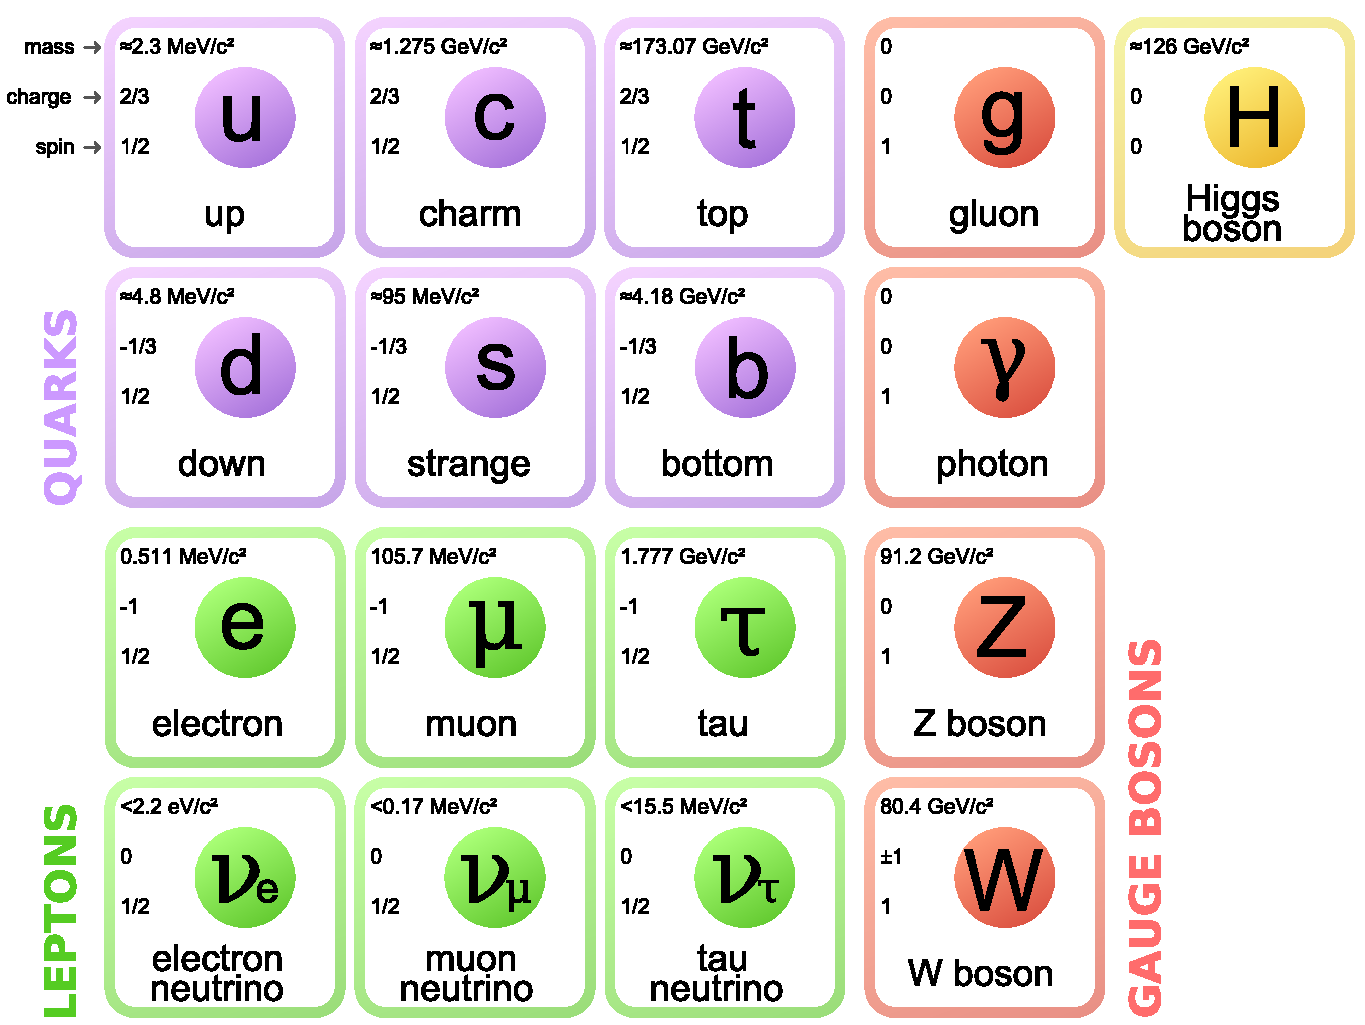
\includegraphics[width=\textwidth]{figures/standard_model.pdf}
    \caption[
        The particles of the standard model.
    ]{
        The particles of the standard model with information about their
        type, their mass, charge, and spin. The quarks and leptons make up
        matter, while the gauge bosons mediate interactions. The Higgs gives
        mass to the \W and \Z bosons.
    }
    \label{fig:standard_model}
\end{figure}

There are two types of particles in the standard model: fermions---with half
integer spin---and bosons---with integer spin. The fermions, which make up all
of the matter in the universe, are further subdivided into two groups, leptons
and quarks, while the bosons are divided into gauge bosons and the Higgs.  The
various particles are show schematically in \cref{fig:standard_model}.

Leptons have \spinhalf and have charge $q=-1 \text{ or } 1$ for the massive
leptons, or 0 for the neutrinos. They interact electromagnetically (if they
have a non-zero charge) and weakly. There are three generations of leptons and
each generation consists of a charged, massive lepton, and an uncharged, nearly
massless neutrino. The lightest of the charged lepton generations is the
electron, which is stable. The next two generations contain the muon and the
tau, which are unstable and eventually decay to electrons. The tau, being very
heavy, decays quickly, while the muon is stable long enough to escape a
particle detector. Massive leptons are important in particle detection as they
provide a very clean decay signature. Neutrinos are very difficult to detect in
particle detectors, and so their presence is inferred from the missing energy
in the vector sum of all particles in the collision. This analysis uses
electrons to make its measurement.

Quarks also have \spinhalf although, unlike the leptons, their charge is
fractional and so takes values of $q = 2/3 \text{ or } -1/3$. They interact
strongly, electromagnetically, and weakly. There are three generations of
quarks, with each successive generation having higher mass constituents. The
first generation consists of the up and down (u and d) quarks. These quarks are
stable and make up protons and neutrons, as well as pions. The next generation
of quarks contains the charm and the strange (c and s). They form heavier
states that decay quickly like the \jpsi and kaons. The final generation
consist of the heavy bottom (b), and the exteriorly heavy top (t)---the most
massive particle in the standard model. Bottom quarks can form bound states,
but top quarks are so heavy they decay before any bound states can form.

Quarks carry color charge, of which there are three: red (r),
blue (b), and green (g). Strongly interacting objects obey confinement, which
means that only color neutral (colorless) states are allowed. Because of
confinement, quarks bind together into colorless composite particles. These
particles are called mesons---with two quarks (\qqbar)---and baryons---with
three quarks (\baryon). When an object containing quarks breaks up, the
individual colored fragments will create additional colored objects to maintain
their colorless state. This leads to the formation of ``jets'' which are sprays
of high energy particles that originate from one of these fragments as it tries
to maintain its colorless state.

Bosons are the second type of particle in the standard model. They are further
subdivided into gauge bosons---which mediate the three forces---and the Higgs
boson---which gives mass to the \W and \Z bosons.

The gauge boson that mediates the strong force is the gluon. Gluons interact
with objects that carry color, and are themselves carriers of color, allowing
gluons to interact not only with quarks but with other gluons. Gluons can have
any one of eight different possible color-anticolor superpositions that form a
color-octet. This number comes from the number of generators of \SUthree. Such
octets are not unique, but a commonly used definition is listed in
\cref{table:gluon_color}.

% table:gluon_color
\begin{table}[h]
    \centering
    \spacerows{1.2}
    \begin{center}
        \begin{tabular}{c  c}
            %\toprule
            $\left( \xxbar{\red}{\blue} + \xxbar{\blue}{\red} \right) / \sqrt{2}$ &
            $-i \left( \xxbar{\red}{\blue} - \xxbar{\blue}{\red} \right) / \sqrt{2}$ \\
            $\left( \xxbar{\red}{\green} + \xxbar{\green}{\red} \right) / \sqrt{2}$ &
            $-i \left( \xxbar{\red}{\green} - \xxbar{\green}{\red} \right) / \sqrt{2}$ \\
            $\left( \xxbar{\blue}{\green} + \xxbar{\green}{\blue} \right) / \sqrt{2}$ &
            $-i \left( \xxbar{\blue}{\green} - \xxbar{\green}{\blue} \right) / \sqrt{2}$ \\
            $\left( \xxbar{\red}{\red} - \xxbar{\blue}{\blue} \right) / \sqrt{2}$ &
            $\left( \xxbar{\red}{\red} - 2\xxbar{\blue}{\blue} + \xxbar{\green}{\green} \right) / \sqrt{6}$ \\
            %\bottomrule
        \end{tabular}
        \caption[
            One possible QCD color-octet.
        ]{
            One of the possible color-octets. The colors are red (\red), blue
            (\blue), green (\green), and their anticolors ($\overline{\red}$,
            $\overline{\blue}$, and $\overline{\green}$) .
        }
        \label{table:gluon_color}
    \end{center}
\end{table}


There are four gauge bosons that mediate the electroweak interaction: the photon
(\photon), the \Z, and the \Wpm. The photon and the \Z are uncharged, while the
\Wpm carry charge of $\pm1$. The \W and \Z are not the particles described by
the \SUtwoUone group, but are instead linear combinations of these fields
created through combination with the Higgs mechanism. The \W participates in
interactions that change quark and lepton flavor, for example \ttoWb or
\mutoWnu, while the \Z does not.

The \Z boson is an excellent probe of precision physics as its well measured
mass (\Zmass) and its sharp width (\Zwidth) make it easy to identify from its
decay products \cite{pdg2014}. In a hadron collider, the most common \Ztoqq
decay mode is difficult to select as there are many hadronic jets in each
event, and so \Ztoll decay modes are preferred. In this analysis we look at the
\Ztoee decay mode; our collaborators are working on performing a similar
measurement with \Ztomumu decays. A few common decay modes and their branching
fraction are listed in \cref{table:z_decays}.

% table:z_decays
\begin{table}[h]
    \centering
    \spacerows{1.2}
    \begin{center}
        \begin{tabular}{@{}l r@{}}
            \toprule
            Mode         & Fraction $\left( \Gamma_{i} / \Gamma \right)$ \\
            \midrule
            $\Ztoqq$     & $69.91 \pm 0.06\%$ \\
            $\Ztoee$     & $3.363 \pm 0.004\%$ \\
            $\Ztomumu$   & $3.366 \pm 0.007\%$ \\
            $\Ztotautau$ & $3.370 \pm 0.008\%$ \\
            $\Ztonunu$   & $20.00 \pm 0.06\%$ \\
            \bottomrule
        \end{tabular}
        \caption{
            Selected decay modes of the \Z boson.
        }
        \label{table:z_decays}
    \end{center}
\end{table}


The final piece of the standard model, the Higgs boson, gives mass to the weak
bosons through interactions with the Higgs field. In the Lagrangian of the
standard model it is not possible to write a mass term for the bosons
that is gauge invariant. The Higgs mechanism adds a complex scalar field whose
symmetry is spontaneously broken leading to the \W and \Z masses and the
appearance of a \spinzero boson, the Higgs.

\section{\texorpdfstring{\Z}{Z} Boson Transverse Momentum}

The leptonic decays of the \Z are an excellent probe of QCD as neither
the \Z nor the leptons carry color charge. This means that there is no color
flow between the initial and final states, and so the only QCD signature
encoded in the decay of the \Z is that of the initial interaction. One
particularly useful variable for probing QCD is the transverse momentum of the
\Z boson, \bosonpt, where transverse is defined relative to the beamline in the
collider. As the beam protons have near-zero momentum transverse to the
beamline, the \bosonpt of the \Z boson comes from QCD process like initial
state radiation, which are discussed in \cref{ssec:higher_order}. Low
values of \bosonpt probe the non-perturbative regions of QCD as, due to
asymptotic freedom, it is these low momentum transfer interactions where
\alphastrong is large.

In addition aiding in the understanding of QCD processes, measuring the \Z
\bosonpt spectrum helps improve measurements of the \W mass. At a hadron
collider, the best decay channel for measuring the \W mass is \Wtolnu because
the more common \Wtoqq decays are impossible to trigger on. This leaves a
single detected lepton and an undetected neutrino, forcing a fit to be done for
the \pt spectrum of the lepton. Any \bosonpt from the \W adds uncertainty to
this fit, so an accurate measurement of the \W \bosonpt spectrum is needed. As
the \W is subject to the same processes described below for the \Z, the
measurement of the \Z \bosonpt spectrum constrains the \W \bosonpt spectrum.

%\cite{bozzi_2011},
%\cite{mantry_2011}, and \cite{becher_2011}.

\subsection{A New Variable: \texorpdfstring{\phistar}{Phistar}}

In the low \bosonpt region---the region which contains most of the \Z events
and is also the region governed by non-perturbative QCD---the measurement is
dominated by the systematic uncertainties and the experimental resolution.
Theorists have proposed a new variable, \phistar, that depends only on the
direction of the leptons and not on their energy in order to reduce the
systematic uncertainties associated with the measurement \cite{banfi_2011}.
\phistar is correlated to $\bosonpt / \mll$, where $\mll$ is the invariant mass
of the two leptons, so it probes the same physics as \bosonpt. This variable is
less susceptible to detector resolution effects as the energy and momentum
resolutions of a detector are, in general, worse than the position resolution.
This is due to the fact that the position of leptons is measured with a very
fine-grained tracking device whereas the energy is measured with a calorimeter.

The definition of \phistar is:

\begin{equation}\label{eq:phistar}
    \phistar = \COT \frac{\Delta \phi}{2} \SECH \frac{\Delta \eta}{2}
\end{equation}

where $\Delta \phi$ is the azimuthal opening angle between the leptons,
and $\Delta \eta$ is a measure of the scattering angle of the leptons with
respect to the beam direction in the rest frame of the dilepton system.

\ATLAS, one of the other experiments on the Large Hadron Collider (LHC), has
measured \phistar at a center-of-mass energy of $7 \TeV$ (\rootsseven)
\cite{atlas_phistar}. \DZERO has also measured \phistar at the Tevatron at
\rootsTevatron \cite{d0_phistar_2011}\cite{d0_phistar_2014}. This thesis
presents the first measurement of \phistar at \rootseight.

\subsection{\texorpdfstring{\Z}{Z} Boson Differential Cross Section}

The measurement of \phistar that will be performed in this analysis is a
differential cross section measurement. A cross section measurement is, at its
heart, a simple counting experiment. The cross section of a process, $\Z$
production for instance, is given by:

\begin{equation}\label{eq:xsec}
    \sigma \left( \Z \right) = \frac{N_{\Z}}{\luminosity}
\end{equation}

where $N_{\Z}$ is the number of \Z bosons that were created and $\luminosity$
is the integrated luminosity of the data which is a measurement of how many
interaction opportunities took place. A differential cross section is used to
measure the cross section of a process as a function of a variable, for
instance \bosonpt. Then the cross section becomes:

\begin{equation}\label{eq:differ_xsec}
    \frac{\dir{\sigma \left( \Z \right)}}{\dir{\bosonptk} }
    =
    \frac{N_{\Z_{\bosonptk}}}{\Delta \bosonptk \cdot \luminosity}
\end{equation}

where $\bosonptk$ is a range of $\bosonpt$, $N_{\Z_{\bosonptk}}$ is the number
of \Z events with $\bosonpt$ that fall within the range, and $\Delta \bosonptk$
is size of the range. This measurement is still dependent on the luminosity
which can be difficult to accurately measure. This dependency can be removed by
dividing by the total cross section:

\begin{equation}\label{eq:normaized_differ_xsec}
    \frac{1}{\sigma \left( \Z \right)} \frac{\dir{\sigma \left( \Z \right)}}{\dir{\bosonptk} }
    =
    \frac{\luminosity}{N_{Z}} \frac{N_{\Z_{\bosonptk}}}{\Delta \bosonptk \cdot \luminosity}
    =
    \frac{N_{\Z_{\bosonptk}}}{\Delta \bosonptk \cdot N_{Z}}
\end{equation}

\section{Production of \texorpdfstring{\Z}{Z} Bosons In Proton-Proton Collisions}

In order to understand where the transverse momentum of a \Z boson comes from,
it is important to understand how they are produced in the LHC.

\subsection{The Proton Parton Model}
\label{ssec:parton_model}

At the very high energies of the LHC (\rootseight in 2012), a proton is not
well described by assuming that it is composed of only three valence quarks as
the energy of the proton is much higher than its own binding energy ($\approx 1
\GeV$). Instead, it is described by a parton model---a model in which there are
three valence quarks, but also numerous gluons and ``sea quarks'', where the
sea quarks are a superposition of quark and antiquark same-flavor pairs. These
constituents of the protons are referred to as ``partons''.

When two protons collide at the LHC, it is a parton from each that interacts in
the hard scattering process. This parton-parton interaction can be considered
as independent of the other partons as the interaction timescale is short
compared to the size of the proton. Each of the partons that takes place in the
interaction will carry only a faction of their parent proton's total momentum.
This fraction is parameterized by the Bjorken \BjorkenX{i} variable, defined as
$\BjorkenX{i} P = p_{i}$ where $P$ is the total proton momentum and $p_{i}$ is
the momentum of a parton. Most of this momentum is in the same direction as the
beam, but a small fraction of it, less than the proton binding energy of
$1 \GeV$, is transverse to the beamline due to the motion of the partons inside
the proton.

The \BjorkenX{i} value of a parton is not fixed, but is instead a probability
distribution that is dependent on the flavor of the parton and the energy scale
($Q^{2}$) of the interaction. Collections of these distributions for the
various flavors are called parton distribution functions (PDFs). PDFs can not
currently be calculated from QCD, and it is not known if doing so is even
possible. Instead, PDFs are models which are fit to data and extrapolated to
new interaction scales using perturbative QCD. An example set of PDFs from the
MSTW collaboration\cite{martin_2009} is shown in \cref{fig:mstw_pdf}. In
the low interaction energy case, shown on the left plot, the u and the d quark
distributions have peaks at high \BjorkenX{i}, as the valence quarks carry most
of the momentum. In the high interaction energy case, shown on the right plot,
a small peak is still seen in the u and d quark distributions, but the
sea quarks and gluons also carry a large amount of the total momentum.

% fig:mstw_pdf
\begin{figure}[!htb]
    \centering
    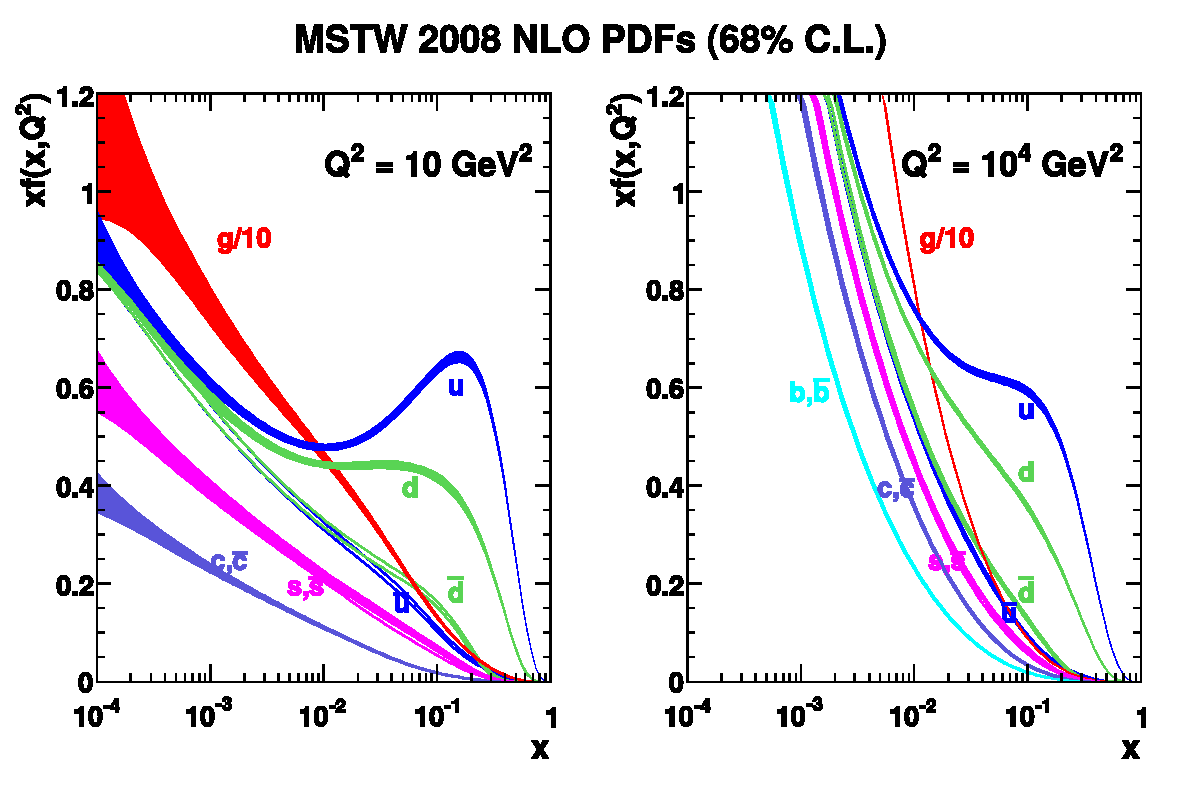
\includegraphics[width=\textwidth]{figures/mstw_pdfs.pdf}
    \caption[
        % \cite{martin_2009}
        Example PDFs from the MSTW collaboration.
    ]{
        Example PDFs from the MSTW collaboration for interaction energy scales
        of $\InteractionEnergy = \SI{10}{\GeV\squared}$ (left) and
        $\InteractionEnergy = \SI{e4}{\GeV\squared}$ (right). The bands
        represent the \BjorkenX{i} distributions for the various partons.
    }
    \label{fig:mstw_pdf}
\end{figure}


\subsection{\DrellYan Production}
\label{ssec:dy_production}

The \DrellYan process is the lowest order in \alphastrong process of producing
dilepton pairs via the \Z boson \cite{drell_1970}\cite{drell_1970a}. The
Feynman diagram of this process is shown in \cref{fig:feyn_s_channel}. As
discussed previously, the two quarks will have $\pt \approx 0$ as most of the
proton's momentum (and hence, the parton's momentum) is along the beamline, and
so the \Z will also have $\bosonpt \approx 0$. The cross section for the
\DrellYan process, in terms of the \BjorkenX{i} variables of the incoming
partons, is:

\begin{equation}\label{eq:drell_yan_cross_section}
    \frac{\dirSquare{\sigma}}
    {\dir{\BjorkenX{1}} \dir{\BjorkenX{2}}}
    =
    \frac{4 \pi \fsc^{2}}
    {9 \BjorkenX{1} \BjorkenX{2} s}
    f \left( \BjorkenX{1}, \BjorkenX{2} \right)
\end{equation}

\begin{equation}\label{eq:fx}
    f \left( \BjorkenX{1}, \BjorkenX{2} \right)
    =
    \sum_{a}
    Q^{2}_{a}
    \left[
        \PDF{a}{1}{\BjorkenX{1}}
        \PDF{\bar{a}}{2}{\BjorkenX{2}}
        +
        \PDF{\bar{a}}{1}{\BjorkenX{1}}
        \PDF{a}{2}{\BjorkenX{2}}
    \right]
\end{equation}

where \BjorkenX{i} is the momentum fraction carried by the parton from the
$i$th proton, \PDF{a}{i}{\BjorkenX{i}} is the individual PDF for a quark of
flavor $a$ from the $i$th proton, $s$ is the Mandelstam variable that is
the square of the center-of-mass energy, and the sum is over quark flavors.

% fig:feyn_s_channel
\begin{figure}[!htbp]
    \centering
    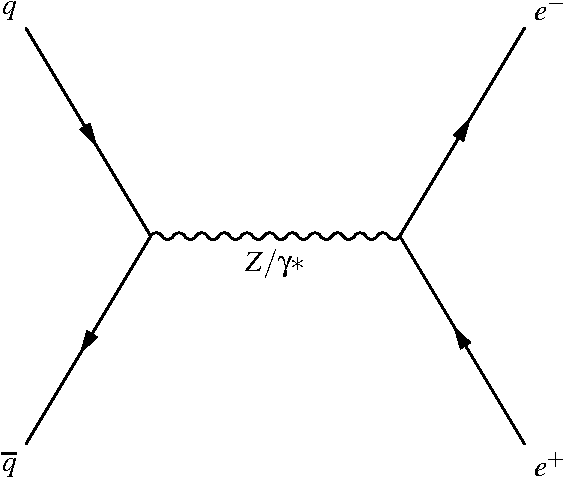
\includegraphics[width=\StackedPlotWidth]{figures/feyn_drell_yan_s_channel.pdf}
    \caption{
       Feynman diagram of \DrellYan \Ztoee production.
    }
    \label{fig:feyn_s_channel}
\end{figure}


\subsection{Higher Order Production}
\label{ssec:higher_order}

In addition to the \DrellYan process discussed previously, there are higher
order terms in \alphastrong that contribute to \Z boson production. Some of
these terms are shown in \cref{fig:higher_order_z_diagrams}.

The first type of term, shown in
\cref{fig:feyn_qqbar_to_zg,fig:feyn_qbarq_to_zg}, contains initial state
radiation (ISR). These diagrams have a gluon radiating from the incoming quark.
This causes the quark to gain momentum equal and opposite to that of the gluon.
The quark will then have some \pt to pass on to the \Z boson. The probability
of radiating a gluon increases as the energy of the radiated gluon decreases,
and so ISR often introduces a small amount of \bosonpt.

The second type of term, shown in
\cref{fig:feyn_qg_to_zq,fig:feyn_qg_to_q_to_zq}, is one where the quark
interacts with a gluon from the other proton and radiates a \Z boson. These
terms, although of order \alphastrong, dominate at that LHC as there is a
larger probability of a gluon being present than an antiquark because the
antiquarks must come from the sea quarks.

% fig:higher_order_z_diagrams
% fig:feyn_qqbar_to_zg, fig:feyn_qbarq_to_zg, fig:feyn_qg_to_zq,
% fig:feyn_qg_to_q_to_zq
\begin{figure}[!p]
    \centering
    \begin{subfigure}[b]{\SideBySidePlotWidth}
        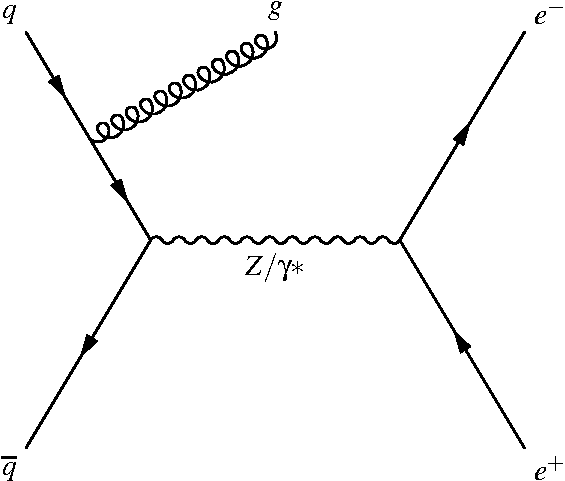
\includegraphics[width=\linewidth]{figures/feyn_qqbar_to_zg.pdf}
        \caption{}
        \label{fig:feyn_qqbar_to_zg}
    \end{subfigure}%
    \begin{subfigure}[b]{\SideBySidePlotWidth}
        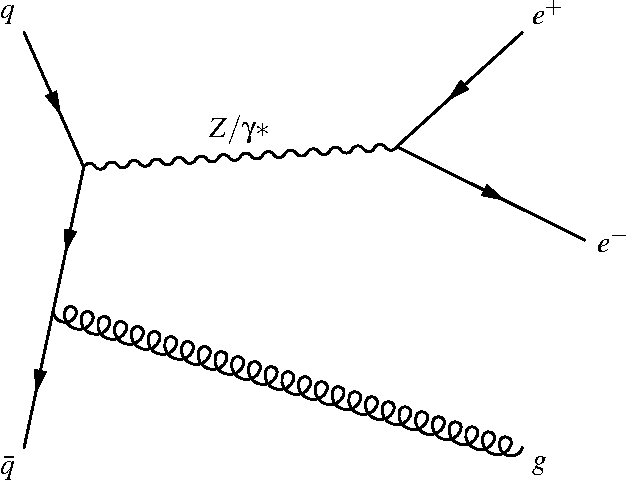
\includegraphics[width=\linewidth]{figures/feyn_qbarq_to_zg.pdf}
        \caption{}
        \label{fig:feyn_qbarq_to_zg}
    \end{subfigure}
    \begin{subfigure}[b]{\SideBySidePlotWidth}
        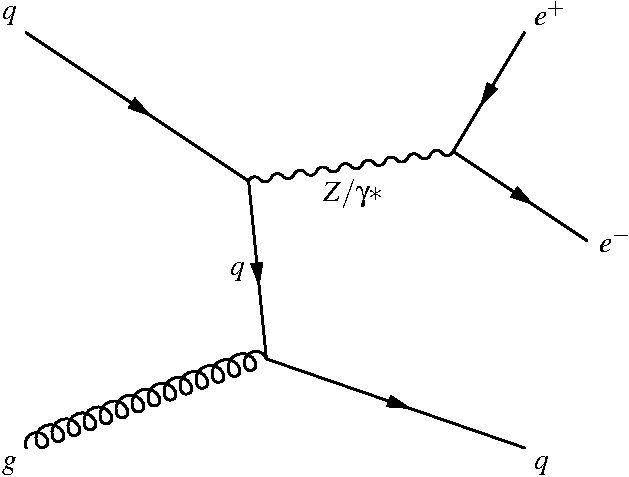
\includegraphics[width=\linewidth]{figures/feyn_qg_to_zq.pdf}
        \caption{}
        \label{fig:feyn_qg_to_zq}
    \end{subfigure}%
    \begin{subfigure}[b]{\SideBySidePlotWidth}
        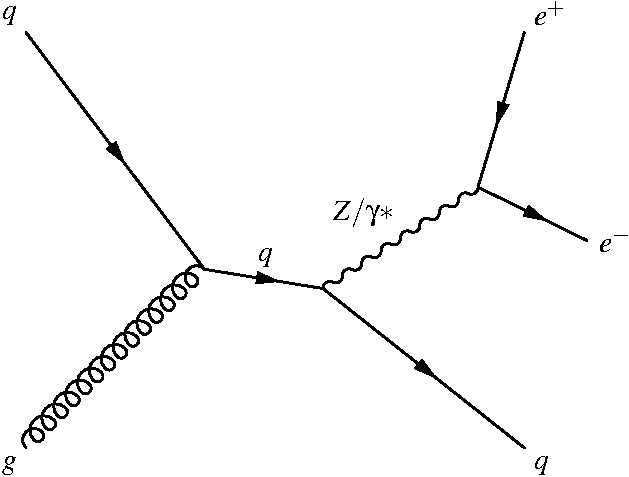
\includegraphics[width=\linewidth]{figures/feyn_qg_to_q_to_zq.pdf}
        \caption{}
        \label{fig:feyn_qg_to_q_to_zq}
    \end{subfigure}
    \caption[
        Higher order in \alphastrong \Ztoee Feynman diagrams.
    ]{
        Higher order in \alphastrong \Ztoee Feynman diagrams. Figures~(a) and
        (b) are ISR where one of the incoming quarks radiates a gluon. In
        \FIGS~(c) and (d) the quark radiates a \Z.
    }
    \label{fig:higher_order_z_diagrams}
\end{figure}


\subsection{Final State Radiation}
\label{sec:electron_dressing}

\begin{figure}[!htb]
    \centering
    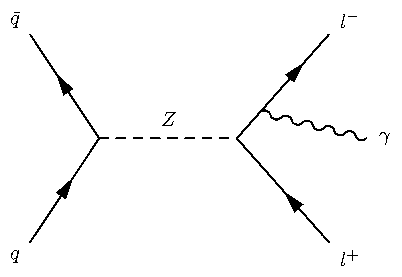
\includegraphics[width=0.65\textwidth]{figures/fsr.pdf}
    \caption{
        Feynman diagram of \Ztoll with FSR.
    }
    \label{fig:fsr_diagram}
\end{figure}

After the \Ztoee decay, the decay electrons can radiate photons in a process
known as final state radiation (FSR). The diagram of this process is shown
in \cref{fig:fsr_diagram}. Different measurements and theories treat FSR
differently, and so we define three types of generator level electron that each
account for FSR in a different manner: \born, \bare, and \dressed.

\Born generator level electrons are electrons directly after the \Ztoee decay
before the electrons have radiated any FSR photons. This definition is what
most theoretical results will provide.

\Bare generator level electrons are \born electrons after they have radiated all
of their FSR photons. This definition most closely matches how muons are
measured in a detector as the momentum of a muon is measured using only its
track, ignoring any photons.

\Dressed generator level electrons are \bare electrons with their FSR photons
added back in vector sum. The photons are only added if they are within a cone
of size $\Delta R < 0.1$ around the electron. This definition most closely
matches how electrons are measured in a detector; the energy of the electron is
measured using a calorimeter which also integrates the nearby photons into the
measurement.

Whenever generator level quantities are used, for example when performing the
unfolding as discussed in \cref{sec:unfolding}, \dressed electrons are
used.

\TODO{We are not going to have bare and born results ready}

\TODO{Whenever generator level quantities are used, for example when performing the
unfolding as discussed in \cref{sec:unfolding}, all three definitions
of generator level electron are used. This allows three final results to be
computed, one with each definition, allowing easy comparison of our results to
other experiments and theoretical models.}
